\PassOptionsToPackage{unicode=true}{hyperref} % options for packages loaded elsewhere
\PassOptionsToPackage{hyphens}{url}
%
\documentclass[ignorenonframetext,]{beamer}
\usepackage{pgfpages}
\setbeamertemplate{caption}[numbered]
\setbeamertemplate{caption label separator}{: }
\setbeamercolor{caption name}{fg=normal text.fg}
\beamertemplatenavigationsymbolsempty
% Prevent slide breaks in the middle of a paragraph:
\widowpenalties 1 10000
\raggedbottom
\setbeamertemplate{part page}{
\centering
\begin{beamercolorbox}[sep=16pt,center]{part title}
  \usebeamerfont{part title}\insertpart\par
\end{beamercolorbox}
}
\setbeamertemplate{section page}{
\centering
\begin{beamercolorbox}[sep=12pt,center]{part title}
  \usebeamerfont{section title}\insertsection\par
\end{beamercolorbox}
}
\setbeamertemplate{subsection page}{
\centering
\begin{beamercolorbox}[sep=8pt,center]{part title}
  \usebeamerfont{subsection title}\insertsubsection\par
\end{beamercolorbox}
}
\AtBeginPart{
  \frame{\partpage}
}
\AtBeginSection{
  \ifbibliography
  \else
    \frame{\sectionpage}
  \fi
}
\AtBeginSubsection{
  \frame{\subsectionpage}
}
\usepackage{lmodern}
\usepackage{amssymb,amsmath}
\usepackage{ifxetex,ifluatex}
\usepackage{fixltx2e} % provides \textsubscript
\ifnum 0\ifxetex 1\fi\ifluatex 1\fi=0 % if pdftex
  \usepackage[T1]{fontenc}
  \usepackage[utf8]{inputenc}
  \usepackage{textcomp} % provides euro and other symbols
\else % if luatex or xelatex
  \usepackage{unicode-math}
  \defaultfontfeatures{Ligatures=TeX,Scale=MatchLowercase}
\fi
% use upquote if available, for straight quotes in verbatim environments
\IfFileExists{upquote.sty}{\usepackage{upquote}}{}
% use microtype if available
\IfFileExists{microtype.sty}{%
\usepackage[]{microtype}
\UseMicrotypeSet[protrusion]{basicmath} % disable protrusion for tt fonts
}{}
\IfFileExists{parskip.sty}{%
\usepackage{parskip}
}{% else
\setlength{\parindent}{0pt}
\setlength{\parskip}{6pt plus 2pt minus 1pt}
}
\usepackage{hyperref}
\hypersetup{
            pdftitle={Toolbox for analysis and prediction of protein and peptide variant effects},
            pdfauthor={Group 3: Felix Pacheco, Jacob Kofoed, Begoña Bolos Sierra, Laura Sans Comerma},
            pdfborder={0 0 0},
            breaklinks=true}
\urlstyle{same}  % don't use monospace font for urls
\newif\ifbibliography
\usepackage{longtable,booktabs}
\usepackage{caption}
% These lines are needed to make table captions work with longtable:
\makeatletter
\def\fnum@table{\tablename~\thetable}
\makeatother
\usepackage{graphicx,grffile}
\makeatletter
\def\maxwidth{\ifdim\Gin@nat@width>\linewidth\linewidth\else\Gin@nat@width\fi}
\def\maxheight{\ifdim\Gin@nat@height>\textheight\textheight\else\Gin@nat@height\fi}
\makeatother
% Scale images if necessary, so that they will not overflow the page
% margins by default, and it is still possible to overwrite the defaults
% using explicit options in \includegraphics[width, height, ...]{}
\setkeys{Gin}{width=\maxwidth,height=\maxheight,keepaspectratio}
\setlength{\emergencystretch}{3em}  % prevent overfull lines
\providecommand{\tightlist}{%
  \setlength{\itemsep}{0pt}\setlength{\parskip}{0pt}}
\setcounter{secnumdepth}{0}

% set default figure placement to htbp
\makeatletter
\def\fps@figure{htbp}
\makeatother


\title{Toolbox for analysis and prediction of protein and peptide variant
effects}
\providecommand{\subtitle}[1]{}
\subtitle{22100 - R for Bio Data Science}
\author{Group 3: Felix Pacheco, Jacob Kofoed, Begoña Bolos Sierra, Laura Sans
Comerma}
\date{Spring 2020}

\begin{document}
\frame{\titlepage}

\begin{frame}

\end{frame}

\begin{frame}{Content}
\protect\hypertarget{content}{}

\begin{itemize}
\tightlist
\item
  Introduction
\item
  Methods

  \begin{itemize}
  \tightlist
  \item
    Data
  \item
    Project overview
  \end{itemize}
\item
  Results
\item
  Discussion
\item
  Conclusion
\end{itemize}

\end{frame}

\begin{frame}{Introduction}
\protect\hypertarget{introduction}{}

Prediction of protein-protein interactions (PPI) are a challenging task.

ML models allow to exploit the content of these PPI data sets.

The aim of this project is to create a toolbox to predict the biological
activity of these peptides with machine learning models.

\begin{itemize}
\tightlist
\item
  Features:

  \begin{itemize}
  \tightlist
  \item
    Support for both sequence or variant input.
  \item
    Support for several sequence encoders.
  \item
    Support for several models.
  \item
    Visualization options.
  \end{itemize}
\end{itemize}

\end{frame}

\begin{frame}{Methods - the data sets}
\protect\hypertarget{methods---the-data-sets}{}

\begin{longtable}[]{@{}lllllll@{}}
\toprule
\begin{minipage}[b]{0.05\columnwidth}\raggedright
\strut
\end{minipage} & \begin{minipage}[b]{0.04\columnwidth}\raggedright
Protein\strut
\end{minipage} & \begin{minipage}[b]{0.14\columnwidth}\raggedright
Target\strut
\end{minipage} & \begin{minipage}[b]{0.12\columnwidth}\raggedright
Biological activity\strut
\end{minipage} & \begin{minipage}[b]{0.08\columnwidth}\raggedright
Species\strut
\end{minipage} & \begin{minipage}[b]{0.08\columnwidth}\raggedright
Num of variants\strut
\end{minipage} & \begin{minipage}[b]{0.30\columnwidth}\raggedright
Score\strut
\end{minipage}\tabularnewline
\midrule
\endhead
\begin{minipage}[t]{0.05\columnwidth}\raggedright
Data set 1\strut
\end{minipage} & \begin{minipage}[t]{0.04\columnwidth}\raggedright
BRCA1\strut
\end{minipage} & \begin{minipage}[t]{0.14\columnwidth}\raggedright
BARD1 RING domain\strut
\end{minipage} & \begin{minipage}[t]{0.12\columnwidth}\raggedright
Ubiquitin E3 activity\strut
\end{minipage} & \begin{minipage}[t]{0.08\columnwidth}\raggedright
\emph{H. sapiens}\strut
\end{minipage} & \begin{minipage}[t]{0.08\columnwidth}\raggedright
5610\strut
\end{minipage} & \begin{minipage}[t]{0.30\columnwidth}\raggedright
Y2H assays\strut
\end{minipage}\tabularnewline
\begin{minipage}[t]{0.05\columnwidth}\raggedright
Data set 2\strut
\end{minipage} & \begin{minipage}[t]{0.04\columnwidth}\raggedright
ERK2\strut
\end{minipage} & \begin{minipage}[t]{0.14\columnwidth}\raggedright
Small molecule (SCH772984)\strut
\end{minipage} & \begin{minipage}[t]{0.12\columnwidth}\raggedright
Resistance to drugs\strut
\end{minipage} & \begin{minipage}[t]{0.08\columnwidth}\raggedright
\emph{H. sapiens}\strut
\end{minipage} & \begin{minipage}[t]{0.08\columnwidth}\raggedright
6810\strut
\end{minipage} & \begin{minipage}[t]{0.30\columnwidth}\raggedright
Drug sensitivity assays. Calculation of cell availability\strut
\end{minipage}\tabularnewline
\begin{minipage}[t]{0.05\columnwidth}\raggedright
Data set 3\strut
\end{minipage} & \begin{minipage}[t]{0.04\columnwidth}\raggedright
LDLRAP1\strut
\end{minipage} & \begin{minipage}[t]{0.14\columnwidth}\raggedright
OBFC1\strut
\end{minipage} & \begin{minipage}[t]{0.12\columnwidth}\raggedright
Protein translation\strut
\end{minipage} & \begin{minipage}[t]{0.08\columnwidth}\raggedright
\emph{H. sapiens}\strut
\end{minipage} & \begin{minipage}[t]{0.08\columnwidth}\raggedright
6385\strut
\end{minipage} & \begin{minipage}[t]{0.30\columnwidth}\raggedright
Y2H assays\strut
\end{minipage}\tabularnewline
\begin{minipage}[t]{0.05\columnwidth}\raggedright
Data set 4\strut
\end{minipage} & \begin{minipage}[t]{0.04\columnwidth}\raggedright
Pab1\strut
\end{minipage} & \begin{minipage}[t]{0.14\columnwidth}\raggedright
el4FG1\strut
\end{minipage} & \begin{minipage}[t]{0.12\columnwidth}\raggedright
Translation initiation\strut
\end{minipage} & \begin{minipage}[t]{0.08\columnwidth}\raggedright
\emph{S. cereviseae}\strut
\end{minipage} & \begin{minipage}[t]{0.08\columnwidth}\raggedright
1340\strut
\end{minipage} & \begin{minipage}[t]{0.30\columnwidth}\raggedright
Y2H assays\strut
\end{minipage}\tabularnewline
\bottomrule
\end{longtable}

\end{frame}

\begin{frame}[fragile]{Methods - packages used}
\protect\hypertarget{methods---packages-used}{}

\begin{verbatim}
library("tidyverse")
library("dplyr")
library("devtools")
library("Peptides")
library("ggseqlogo")
library("UniprotR")
library("neuralnet")
library("keras")
\end{verbatim}

\end{frame}

\begin{frame}{Example data set 1 - data overview}
\protect\hypertarget{example-data-set-1---data-overview}{}

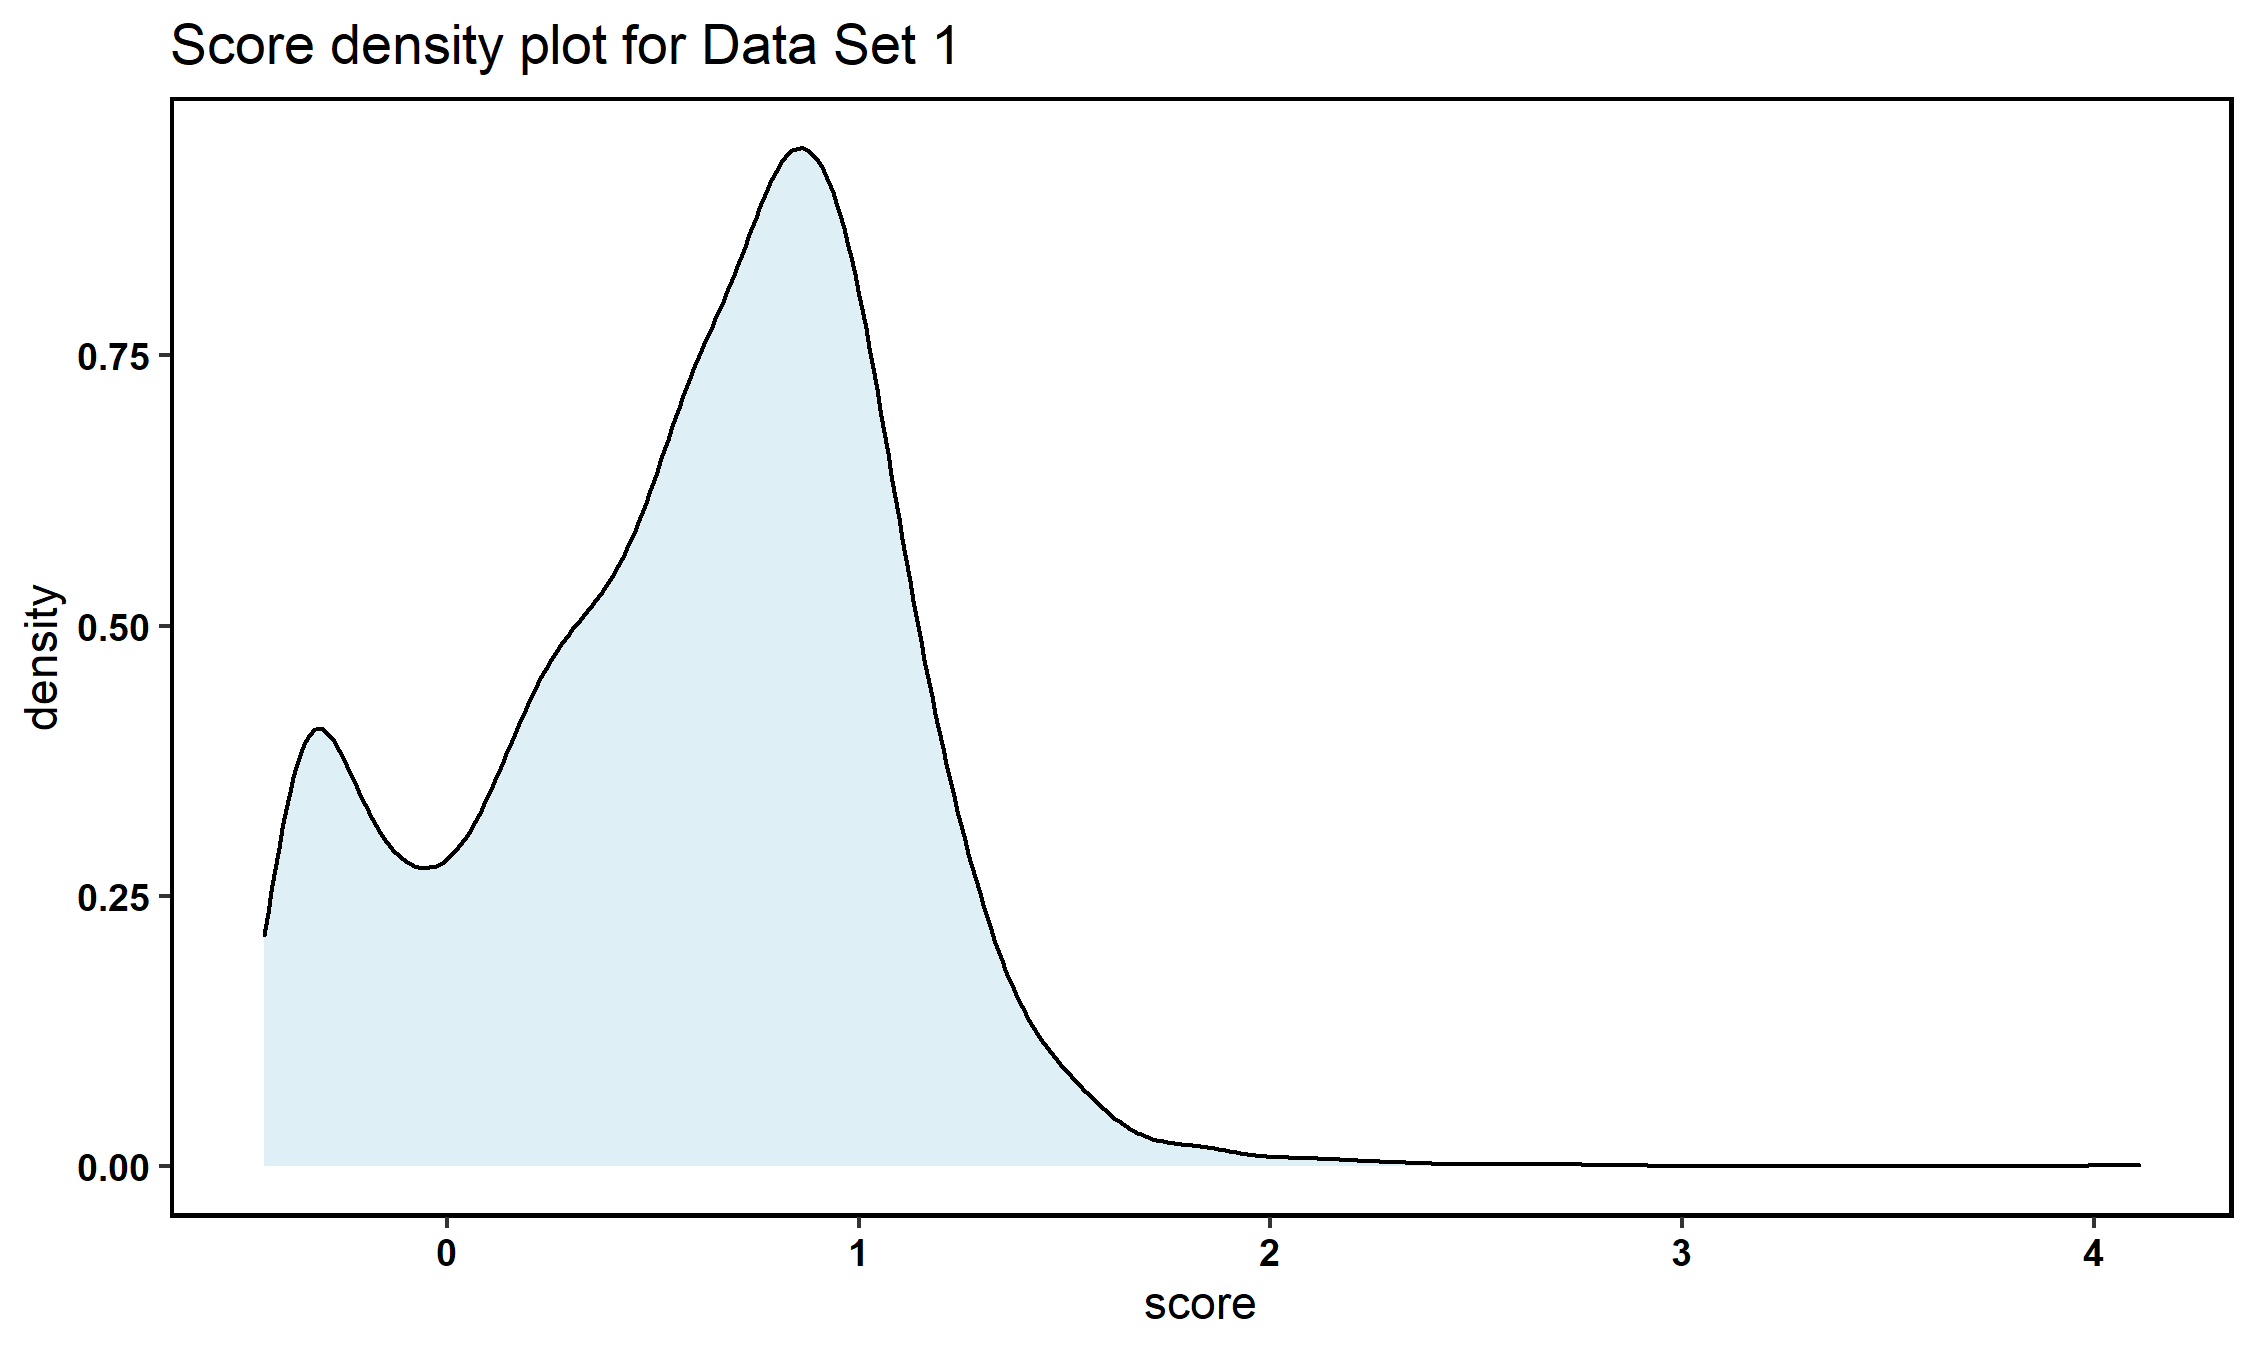
\includegraphics[width=1\textwidth,height=\textheight]{density_plots/density_data_set_1.png}

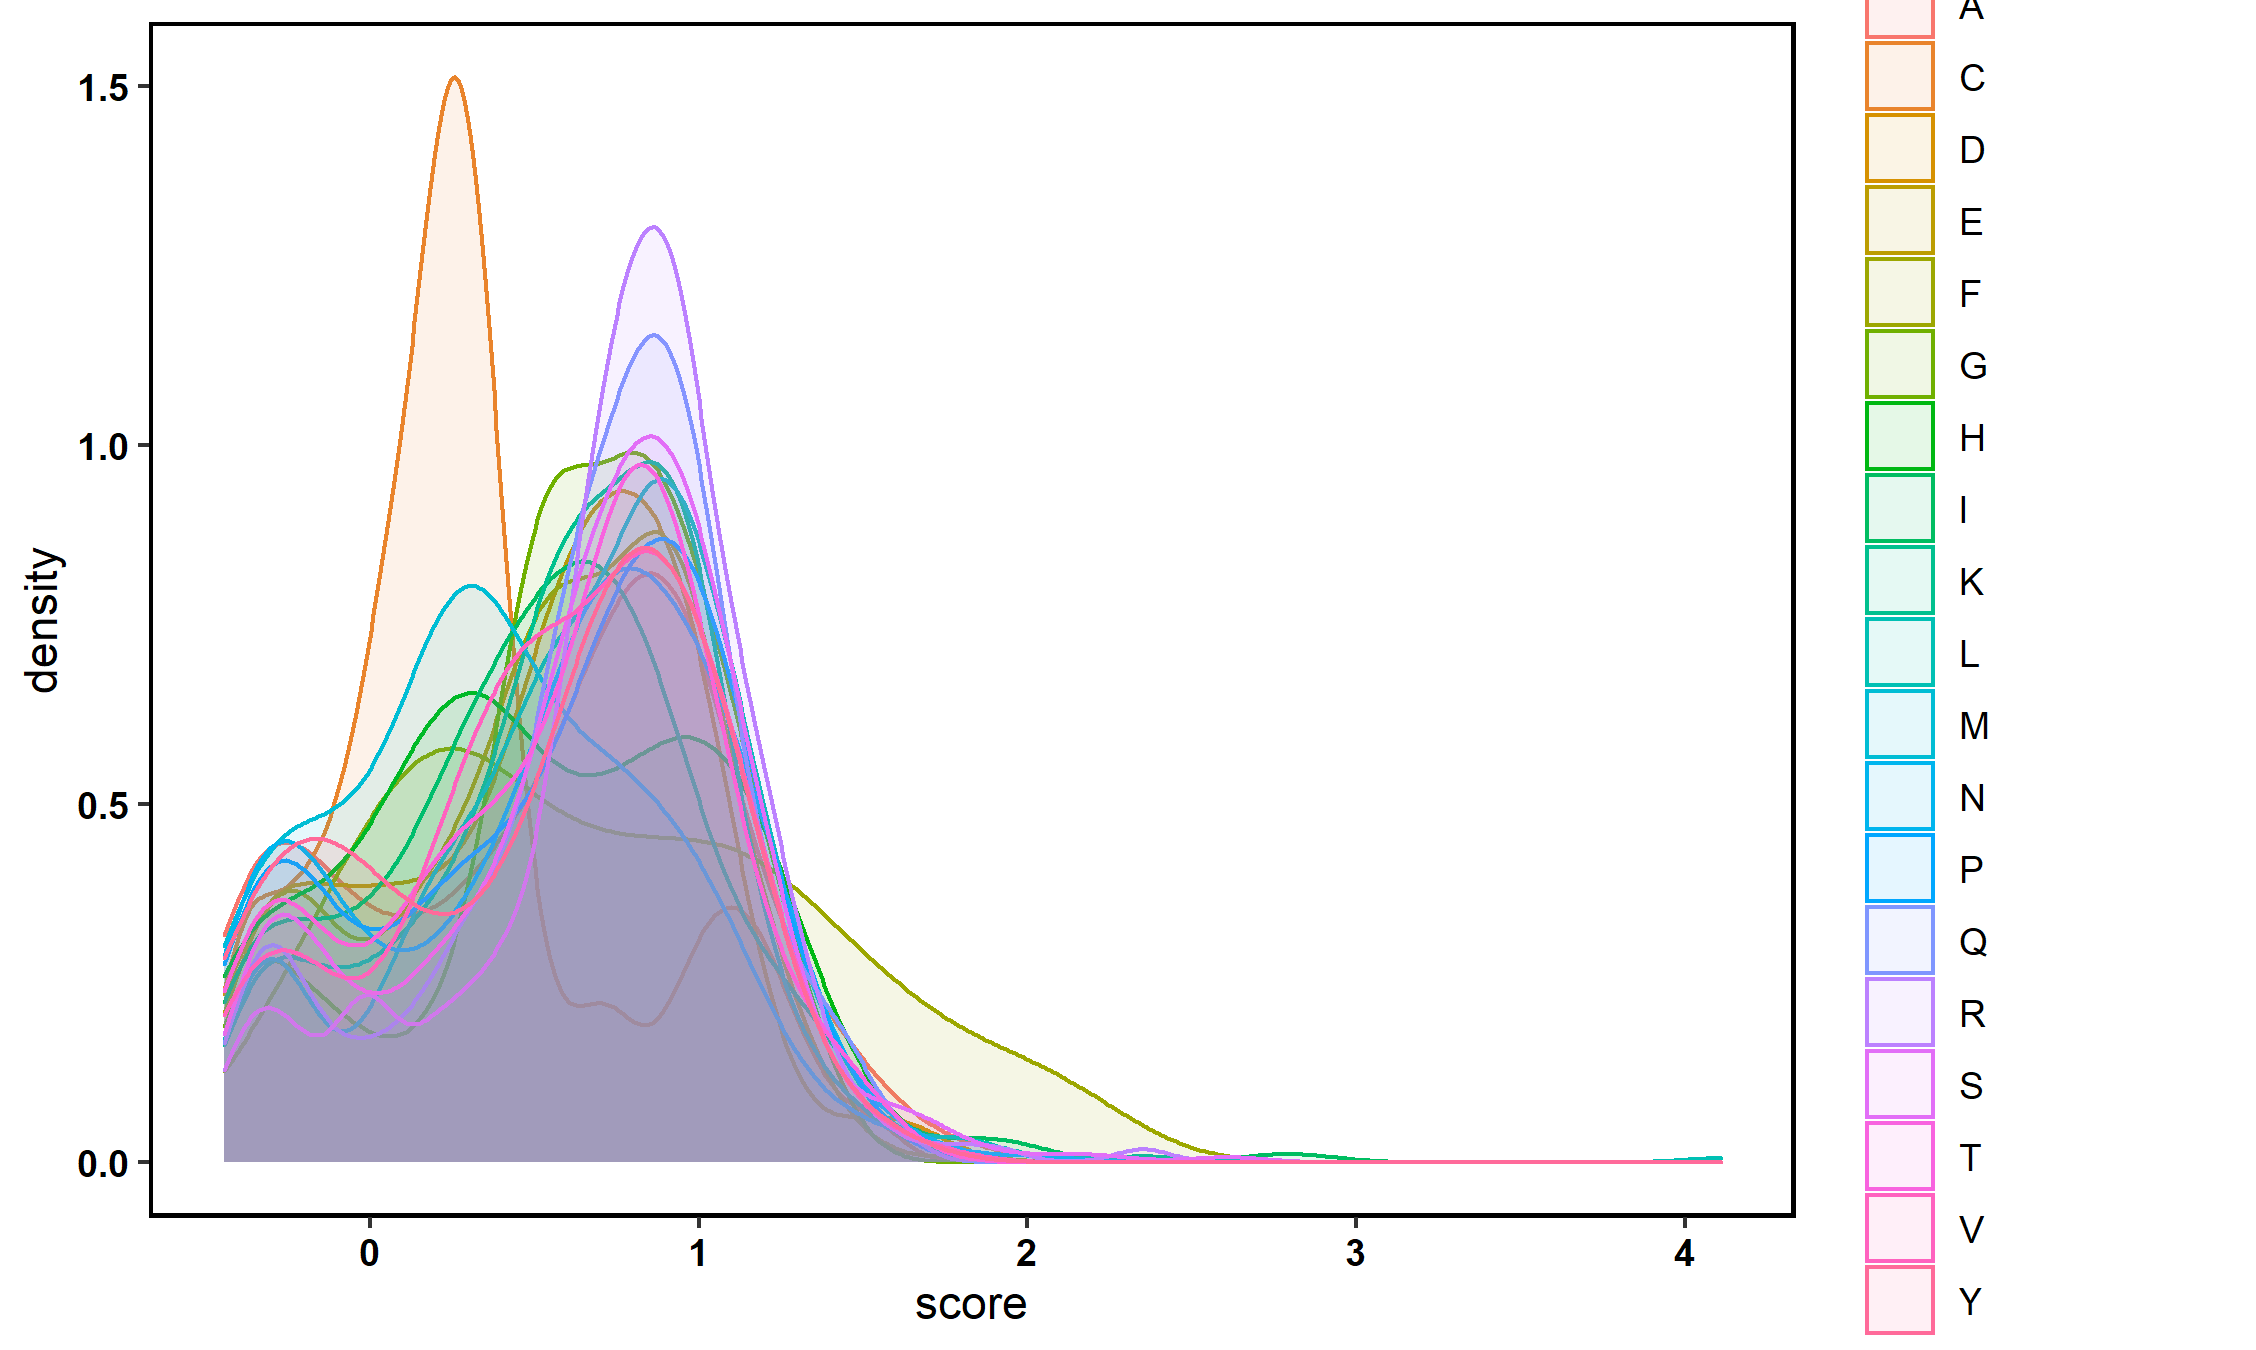
\includegraphics[width=1\textwidth,height=\textheight]{density_plots/density_residue_data_set_1.png}

\end{frame}

\begin{frame}{Example dataset 1 - heatmap}
\protect\hypertarget{example-dataset-1---heatmap}{}

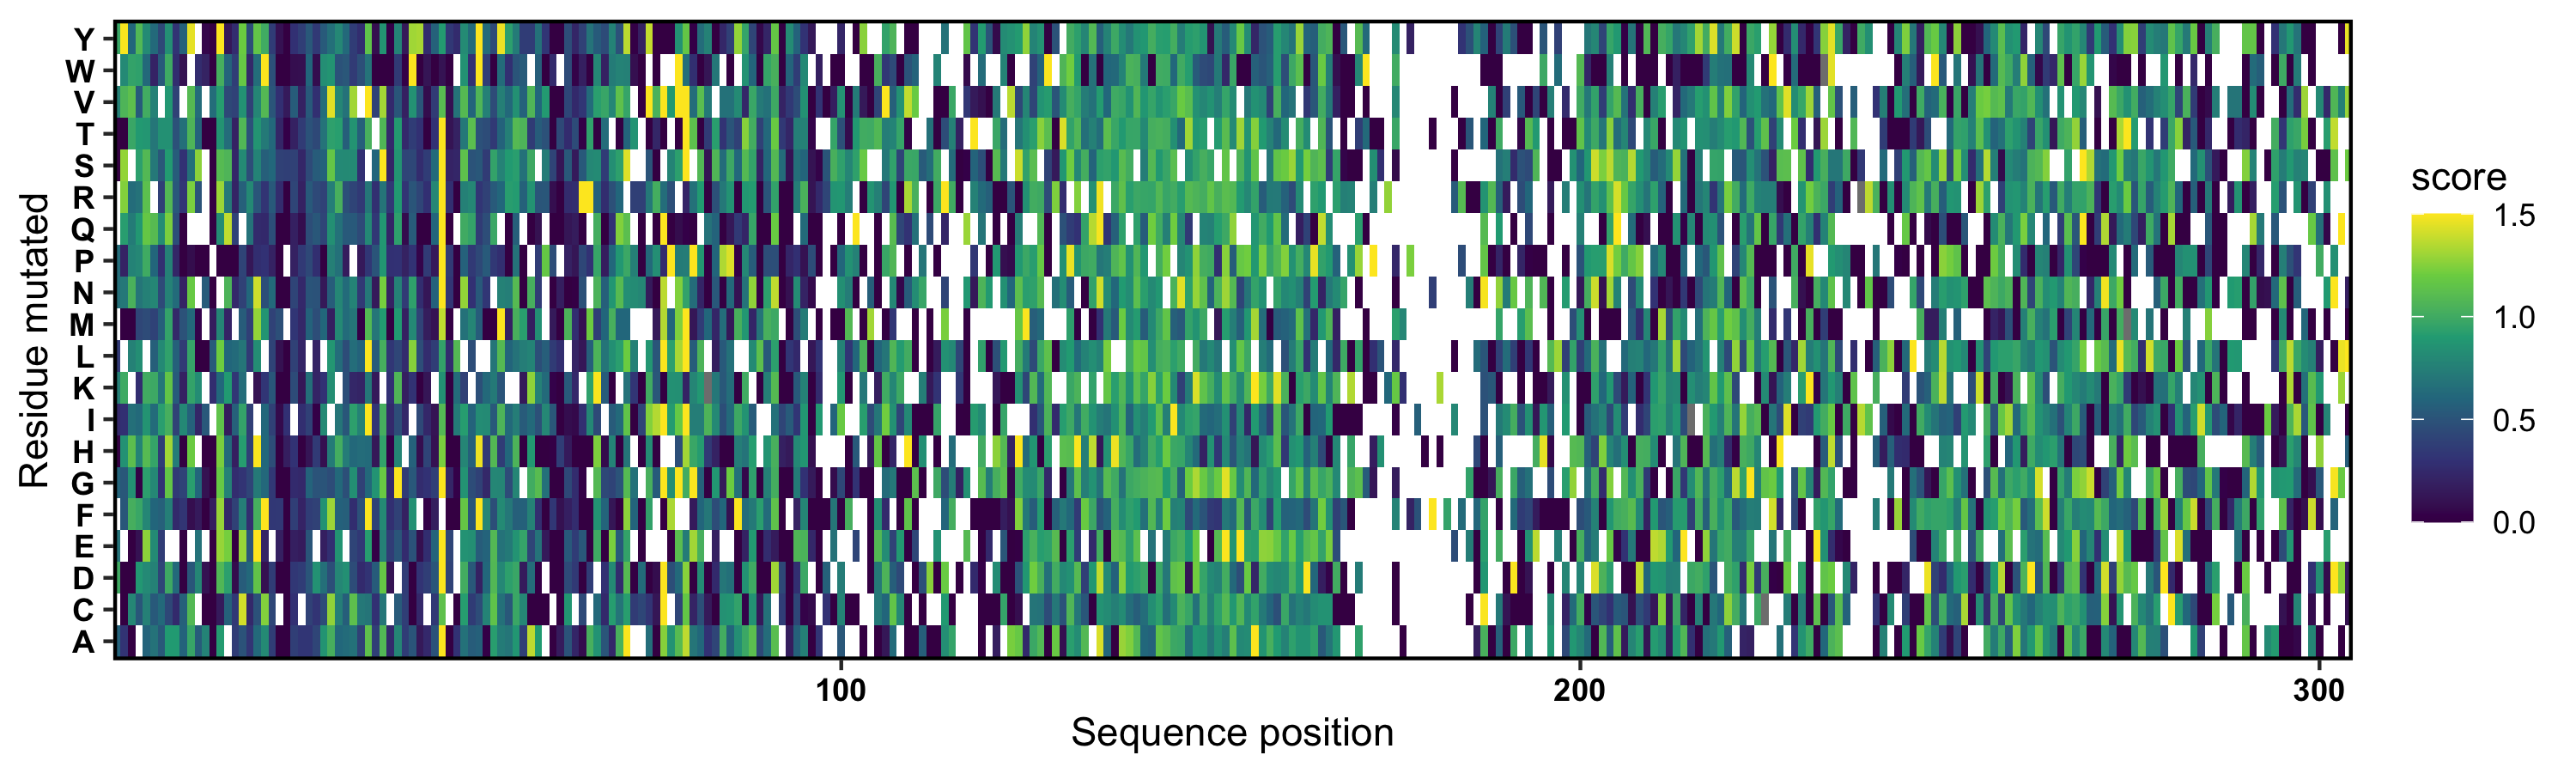
\includegraphics[width=1\textwidth,height=\textheight]{heatmaps/heatmap_data_set_score_1.png}

\end{frame}

\begin{frame}{Example dataset 1 - conserved regions}
\protect\hypertarget{example-dataset-1---conserved-regions}{}

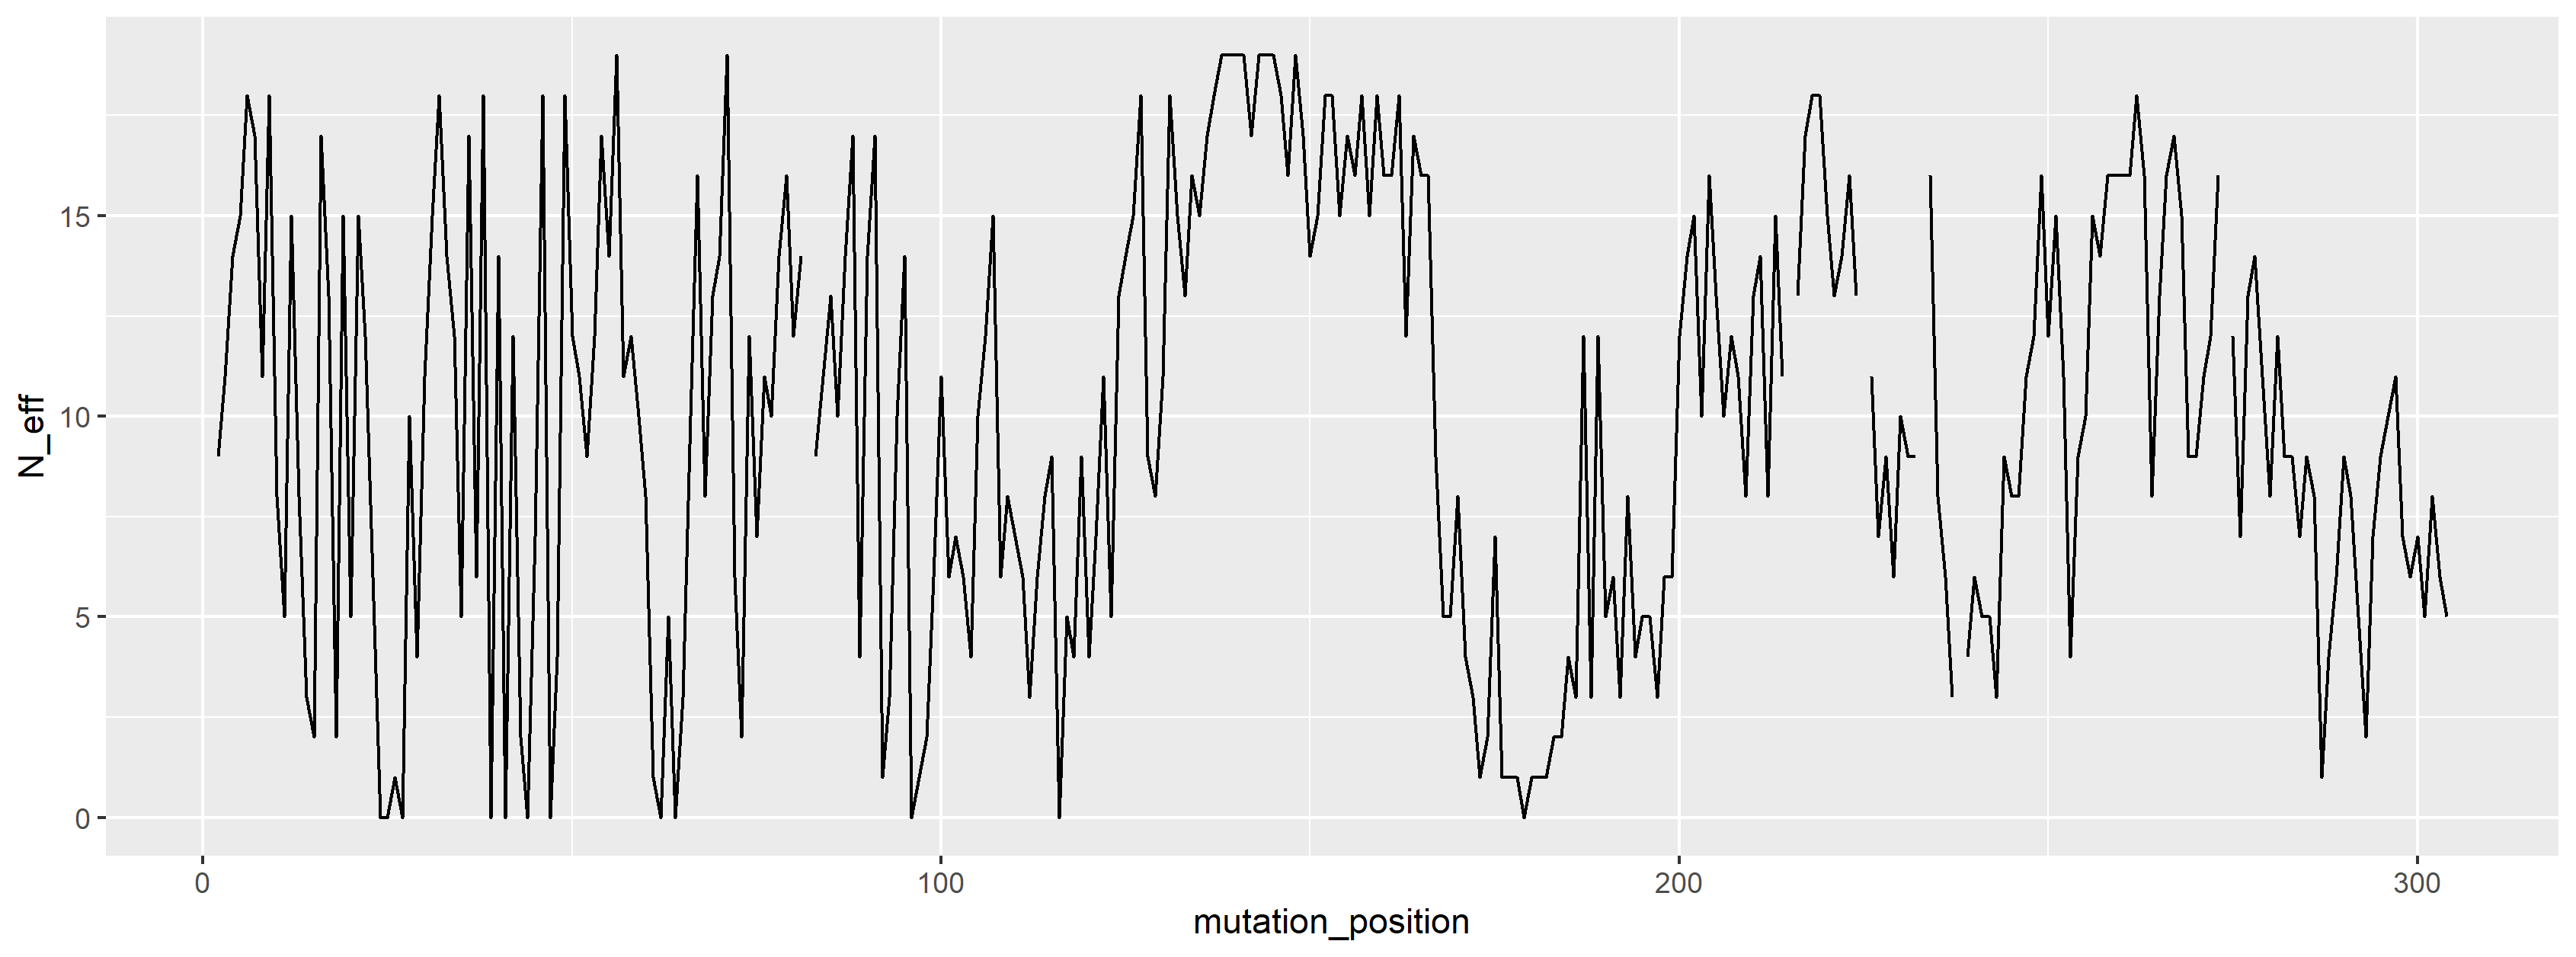
\includegraphics[width=1\textwidth,height=\textheight]{quick_SAR/quick_sar_data_set_1.png}

\end{frame}

\begin{frame}{Machine learning toolbox}
\protect\hypertarget{machine-learning-toolbox}{}

\begin{itemize}
\item
  Ideas for supported machine learning framework:

  \begin{itemize}
  \tightlist
  \item
    Gaussian Process Regression.
  \item
    Artificial Neutral Network.
  \item
    ElasticNet Regression.
  \end{itemize}
\end{itemize}

\end{frame}

\begin{frame}{Results}
\protect\hypertarget{results}{}

\end{frame}

\begin{frame}{Conclusion}
\protect\hypertarget{conclusion}{}

\end{frame}

\begin{frame}{Referencex}
\protect\hypertarget{referencex}{}


\includegraphics[width=3.125in,height=\textheight]{/figures_presentation/file.png}

\begin{itemize}
\tightlist
\item
  \textbf{Data set 1}: L. M. Starita, D. L. Young, et al.
  \emph{Massively parallel functional analysis of brca1 ring
  domainvariants}, Genetics, vol.~200, no. 2, pp.~413--422, 2015. 
\item
  \textbf{Data set 2}: L. Brenan, A. Andreev, et al. \emph{Phenotypic
  characterization of a comprehensive set of missense mutants}. Cell
  Reports, vol.~17, no. 4, pp.~1171--1183, 2016. 
\item
  \textbf{Data set 3}: A deep mutational scan of LDLRAP1 based on a Y2H
  assay with the interactor OBFC1.
  {[}\url{https://www.mavedb.org/scoreset/urn:mavedb:00000036-a-1/}{]} 
\item
  \textbf{Data set 4}: D. Melamed, D. L. Young, et al. \emph{Combining
  natural sequence variation withhigh throughput mutational data to
  reveal protein interaction sites}. PLOS Genetics, vol.~11, no.
  2,pp.~1--21, 2015. 
\end{itemize}

\end{frame}

\begin{frame}[fragile]{Appendix}
\protect\hypertarget{appendix}{}

\begin{block}{R script overview 1}

\begin{verbatim}
data_set_1 <- read_tsv(file = './data/_raw/loaded_data_1.tsv')


# Data_set 1
# select variant_ID and activity to predict

data_set_1_clean <- data_set_1 %>%
  select(Variant_ID, E3_score) %>%
  rename(
  variant = Variant_ID,
  score = E3_score
  ) %>%
  filter(!str_detect(variant, "\\*"))
\end{verbatim}

\begin{itemize}
\tightlist
\item
  02\_clean.R

  \begin{itemize}
  \tightlist
  \item
    Load: Load data from 01\_load.R
  \item
    Wrangle data: Remove NaN, fixes
  \item
    Save cleansed data in .tsv format
  \end{itemize}
\item
  03\_augment.R

  \begin{itemize}
  \tightlist
  \item
    Load data from 02\_clean.R
  \item
    Augment data: Calculate sequences, descriptors, properties
  \item
    Save augmente data in .tsv format
  \end{itemize}
\end{itemize}

\end{block}

\end{frame}

\begin{frame}{Appendix}
\protect\hypertarget{appendix-1}{}

\begin{block}{R script overview 2}

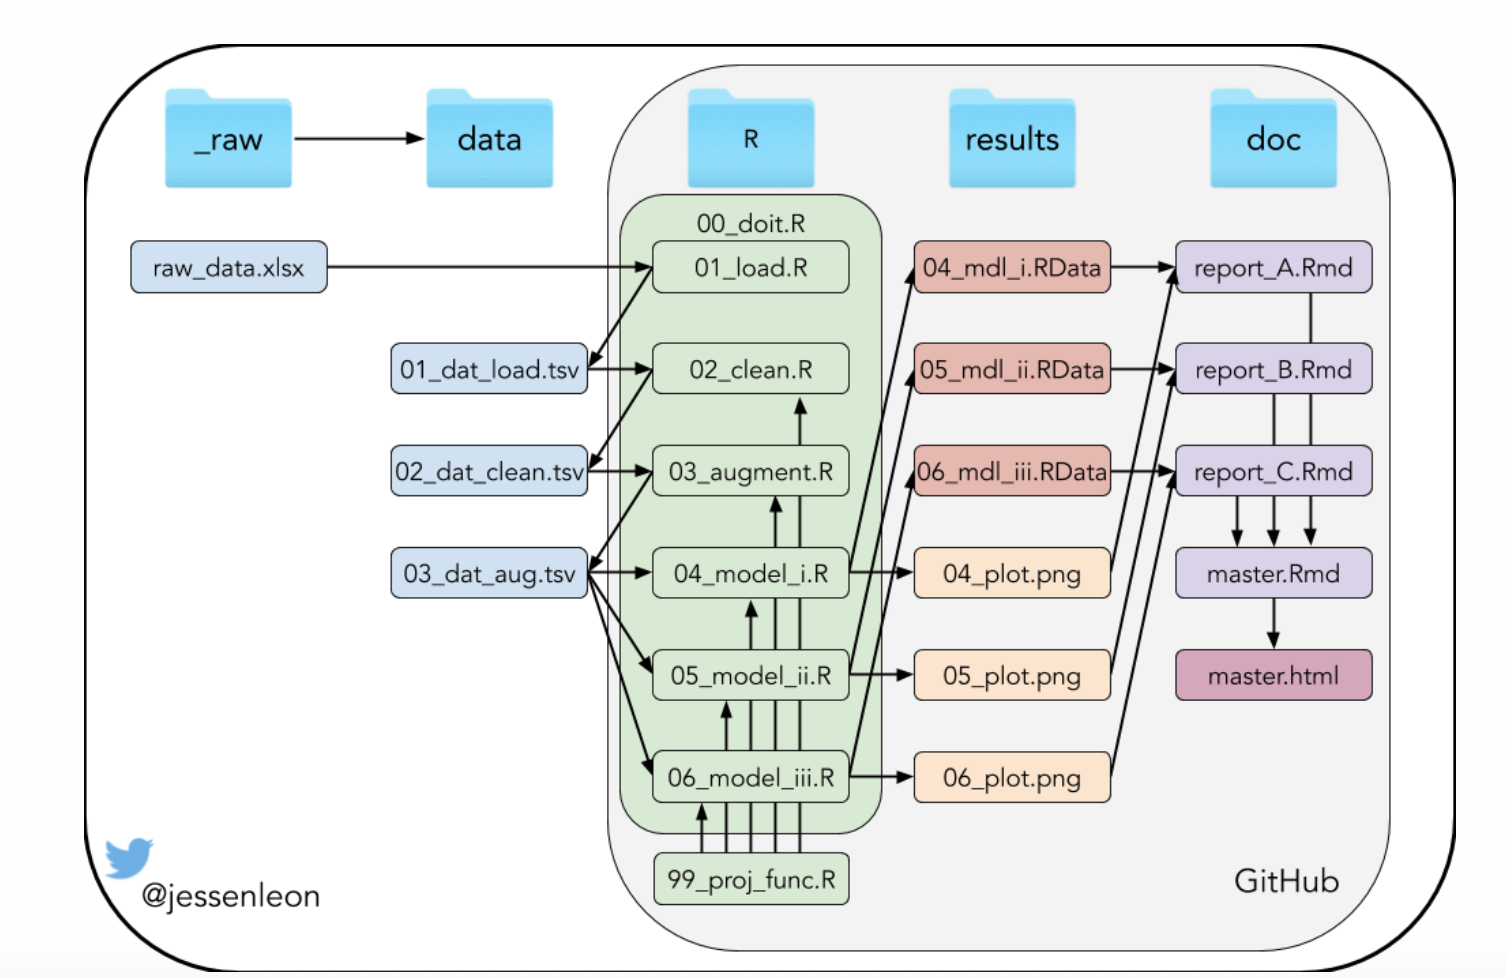
\includegraphics[width=5.20833in,height=\textheight]{project_organisation.png}

\begin{itemize}
\tightlist
\item
  04\_model\_i.R

  \begin{itemize}
  \tightlist
  \item
    Load augmented data
  \item
    Perform model fitting
  \item
    Predict unknowns
  \item
    Plotting and reporting
  \end{itemize}
\end{itemize}

\end{block}

\end{frame}

\begin{frame}{Appendix}
\protect\hypertarget{appendix-2}{}

\begin{block}{R script overview 3}

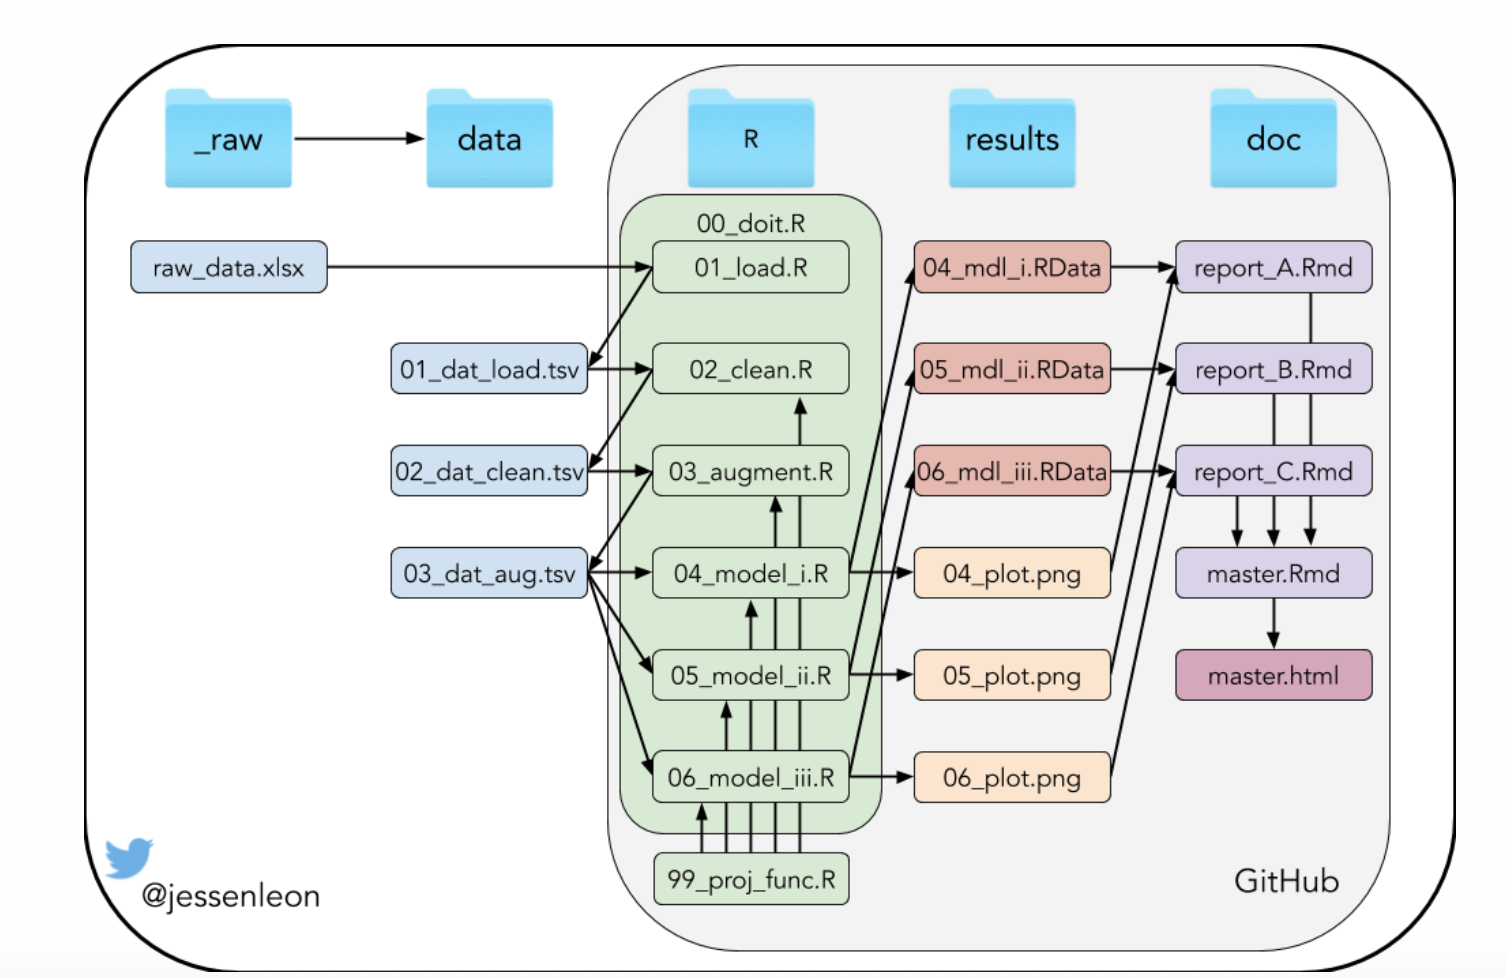
\includegraphics[width=5.20833in,height=\textheight]{project_organisation.png}

\begin{itemize}
\tightlist
\item
  99\_proj\_func.R

  \begin{itemize}
  \tightlist
  \item
    Sequence encoder
  \item
    Sequence generator
  \item
    \ldots{}
  \end{itemize}
\end{itemize}

\end{block}

\end{frame}

\end{document}
